\addcontentsline{toc}{section}{Abstract}
\section*{Abstract} Land-use change is a major driver of biodiversity loss. Land-use change globally impacts vertebrate ecological communities by reducing local species richness. Nevertheless, not all species respond similarly to land-use change. Species ability to cope with anthropogenic pressures is dependent on their functional traits. By preferentially removing certain functional types, land-use change is reshaping the functional composition of ecological communities. Nevertheless, there is no assessment to date of how global land-use change impacts the functional diversity of local vertebrate communities. 

Here, I used a meta-analytic approach to investigate how land-use change impacts the functional diversity of terrestrial vertebrate communities at global scales. Specifically, I used seven vertebrate traits to estimate the functional richness of 6758 local vertebrate communities located worldwide in eight different land-uses, as well as the functional dispersion and functional redundancy for 5554 sites. Using mixed-effect models, I estimated the effects of land-use on each functional diversity index.  

Land-use change globally promotes the functional homogenisation of ecological assemblages by favouring species that share more similar traits values. Disturbed communities are both less functionally dispersed and more functionally redundant. The breadth of functions decreases with increasing human land-use disturbance, as the functional similarity among species increases. As such, land-use change induces the functional clustering of local vertebrate assemblages, with  potential impacts on local ecosystem processes remaining largely unknown.

\pagebreak


\section{Introduction}
Global biodiversity is facing unprecedented challenges \citep{Pereira2012, Newbold2019_ets}. In the past decades, vertebrate populations have declined by 60\% \citep{LivingPlanetIndex2018}. Rates of ongoing extinctions exceeds those inferred from fossil records \citep{DeVos2015,Barnosky2011, Johnson2017}. This acceleration in biodiversity losses is driven by anthropogenic activities \citep{Steffen2015}. Currently, land-use change is the most important of the diverse anthropogenic pressures driving global biodiversity losses \citep{Newbold2015, Foley2005}. Future projections show that land-use change, alongside climate change, is likely to remain one of the major threats on biodiversity \citep{Newbold2018}. To enforce efficient conservation measures, it is vital to consolidate our understanding of how land-use change will impact the diversity of ecological communities. Moreover, it is now widely acknowledged that biodiversity correlates with  ecosystem functioning and resilience \citep{Tilman2014, Oliver2015, Hooper2012}. As such, species losses are likely to provoke disturbances in ecosystem functioning, which could ultimately negatively impact the services ecosystems provide, many of which are fundamental for human well-being \citep{MEA2005}. 

One way to is to characterise ecosystem functioning is to assess the trait composition of ecological communities. Indeed, species can be viewed as a collection of traits that determine species fundamental and realised niches, and that underpin their ecological roles \citep{Violle2007, Cadotte2011}. Functional diversity indices aim at describing the diversity and variability of species functional traits.

In the recent years, diverse indices have been developed to quantify functional diversity \citep{Schleuter2010, Legras2018, Villeger2008, Ricotta2016, Botta-Dukat2009, Laliberte2010}. The quantification of functional diversity can thus inform on processes beyond what other measures of biodiversity (such as species richness) can offer \citep{Cadotte2011, Laureto2015}. The diverse metrics that have been developed aim at capturing different facets of functional diversity. For instance, the functional richness index developed by \citet{Petchey2002} focuses on estimating the total functional distance among species in a community. The functional dispersion index proposed by \citet{Laliberte2010} quantifies the variability in the trait composition of a given community. 

Traits are hence central to the calculation of functional diversity indices. In particular, traits that underpin ecosystem processes are termed `effect traits' \citep{Lavorel2002}. Modification in the effect trait composition of a community can lead to changes in ecosystem functioning \citep{Seguin2014, DeBello2010}. By measuring facets of biodiversity that can directly link to ecosystem processes, functional indices are particularly relevant to understand how disturbances may impact ecosystem functioning. In that case, functional diversity is used as a proxy for ecosystem functioning. Studies investigating how changes in biodiversity relate to changes in ecosystem functioning, using species traits as a mechanistic link, have been mostly focused on plant and invertebrate communities \citep{Hevia2017}. As emphasized by \citet{Cadotte2011}, for functional indices to be strictly informative of ecosystem functions, they should be based on traits that have explicit links with ecosystem functioning (or effect traits).

As opposed to effect traits, `response traits' qualify traits that influence how species respond to disturbances \citep{Lavorel2002}. For instance, empirical evidence has shown that bigger tetrapods are more sensitive to land-use change pressures than smaller tetrapods \citep{Rapacciuolo2017}. As such, body mass has been identified as a response trait to land-use change in terrestrial vertebrates. Diverse studies have documented changes in the trait composition of vertebrate communities affected by land-use change by or habitat degradation \citep{Newbold2014, Colin2018, LaSorte2018, Flynn2009, Tinoco2018}. Such studies provide with empirical evidence that land-use change leads to non-random modifications of the functional composition of vertebrates. Functional diversity indices can therefore reflect changes in functional composition due to the uneven sensitivity of species, underpinned by their response traits. 

Functional diversity indices are therefore useful to investigate how a disturbance affects the trait composition of ecological communities. Whether functional metrics explicitly link to ecosystem functions depends partly on the set of traits included in the calculation. When response and effect traits are coupled, changes in the functional composition of a community triggered by environmental drivers mirrors potential changes in ecosystem functioning. On the other hand, when effect and response traits are uncoupled, shifts in the functional composition of a community do not directly reflect changes in ecosystem processes \citep{Luck2013}. In terrestrial vertebrates, studies that investigated the impacts of land-use change on the functional diversity of ecological communities mostly used a set of traits that related to key ecosystem roles; traits notably related to species resource use and energy transfers. For instance, \citet{Flynn2009} showed that land-use intensification (from natural to agricultural) constricted the functional richness of over 25\% mammalian and avian communities in the temperate Americas. Nevertheless, to my knowledge, no study has yet investigated how land-use change impacts the functional diversity of terrestrial vertebrates at global scales, across the four classes. Investigating this question is central to understand of global land-use change is reshaping the composition of ecological communities, and how these changes could relate to ecosystem functioning.

In this work, I aimed to assess how land-use change impacts the functional diversity of local terrestrial vertebrate communities at global scales. Specifically, I quantified functional richness (the breadth of functions), functional dispersion and functional redundancy (the two latter metrics characterising how functionally similar species are).
I used a meta-analytic approach, based upon the PREDICTS database \citep{Hudson2014, Hudson2017}, to test the following hypotheses:
\begin{itemize}
\item \textbf{Land-use change leads to decreases in the functional richness of local vertebrate communities.} The range of ecological roles decreases in more disturbed land-uses. Land-use change homogenises the local environment and as such acts as an environmental filter. Species presenting certain traits are not able to persist in disturbed habitats and are selectively removed. Previous work has shown that larger, longer-lived species are more sensitive to land-use change \citep{Newbold2013}. Therefore, I hypothesise that the range of functions is likely to be constricted in disturbed habitats compared to natural habitats. 
\item \textbf{The functional dispersion of vertebrate communities decreases with increasing land-use disturbance.} Species in disturbed habitats are more functionally similar than species in more pristine environments, as a consequence of hypothesis (1): species presenting more extreme trait values are being removed from disturbed land-uses, so that remaining species overall have more similar functional roles in disturbed habitats than in more pristine habitats. 
\item\textbf{The functional redundancy of vertebrate communities increases with increasing land-use disturbance.} As species in more disturbed habitats are more functionally similar than species in more pristine environments (hypothesis 2), more species are functionally redundant in disturbed habitats than in pristine environment. With an increase in species richness, new functional roles are introduced at higher rates in pristine environments than in disturbed habitats (see Figure \ref{fredundancy_ltr} in Chapter 1). The increase in functional redundancy is intrinsically coupled with the decrease in functional dispersion. 
\end{itemize}


\section{Methods}

\subsection{The PREDICTS database: using a `space-for-time' substitution to assess the impacts of land-use change on local vertebrate communities}
The impacts of land-use change on the functional diversity of vertebrate communities were assessed using a `space-for-time' substitution \citep{depalma2018}. A longitudinal approach would require data on the evolution of local community composition as the landscape changes from pristine to disturbed, with experimental designs such as `before-after-control-impact' \citep{depalma2018}. Nevertheless, such data are difficult to obtain at large scales for diverse taxa and for multiple types of environmental change. With the space-for-time substitution, a spatial gradient is used as a proxy for temporal dynamics. This approach facilitates meta-analytic studies, as data on the community composition of local assemblages in various land-uses is both easier to collect and more abundant. 

Such data were compiled in the PREDICTS database \citep{Hudson2014, Hudson2017}. This database is the most comprehensive global collection of studies that sampled biodiversity across diverse land-uses. In all studies, species abundance (in most cases) or occurrence was recorded across a variety of sites, each characterised by a land-use (Table \ref{LUcat} and Table \ref{sample_size_LU}). Land-use was divided into six categories: primary vegetation, secondary vegetation, plantation forest, cropland, pasture and urban (Table \ref{LUcat}). Secondary vegetation was further divided in three categories (mature, intermediate and young) according to the stage of recovery of the vegetation. 

\vspace{0.5cm}
\begin{table}[h!]
\renewcommand{\baselinestretch}{1}
\renewcommand{\arraystretch}{1.2}
\begin{center}\fontsize{9}{11}\selectfont
\caption[Land-use categories in the PREDICTS database and their definition.]{\textbf{Land-use categories in the PREDICTS database and their definition.}  See \citet{Hudson2014}, Supplementary Information, for more details. I excluded sites in which land-uses were unknown, as well as secondary vegetation for which the successional stage could not be determined.} 
\label{LUcat}  
\begin{tabular}{|l|l|}
\hline
\multicolumn{1}{|c|}{\textbf{Land-use category}}        & \multicolumn{1}{c|}{\textbf{Definition}}                                                                                                                                                                                                                                                    \\ \hline
Primary vegetation                                      & \begin{tabular}[c]{@{}l@{}}Native vegetation. \\ Undisturbed since its development and stabilisation under current climatic conditions:\\ no known alterations due to human activities or to extreme natural events.\end{tabular}                                                           \\ \hline
Mature secondary vegetation                             & \begin{tabular}[c]{@{}l@{}}Recovering vegetation after complete destruction of primary vegetation\\ (either human activities or natural events), where vegetation succession is complete. \\ The architectural structure is close to that of primary vegetation.\end{tabular}               \\ \hline
\multicolumn{1}{|c|}{Intermediate secondary vegetation} & \begin{tabular}[c]{@{}l@{}}Recovering vegetation after complete destruction of primary vegetation \\ (either human activities or natural events).\\ The architecture is typical of a mid-successional state.\end{tabular}                                                                   \\ \hline
Young secondary vegetation                              & \begin{tabular}[c]{@{}l@{}}Recovering vegetation after complete destruction of primary vegetation\\ (either human activities or natural events). \\ The simple architecture is typical of an early successional state.\end{tabular}                                                         \\ \hline
Plantation forest                                       & \begin{tabular}[c]{@{}l@{}}Previously cleared areas planted with crop trees or shrubs \\ grown and harvested for human consumption or \\ for commercial purposes (includes wood, fruit, oil, biofuel, rubber,...).\end{tabular}                                                             \\ \hline
Pasture                                                 & \begin{tabular}[c]{@{}l@{}}Areas grazed by livestock, permanently or regularly. \\ Can be improved  through cultivation techniques.\end{tabular}                                                                                                                                            \\ \hline
Cropland                                                & \begin{tabular}[c]{@{}l@{}}Previously cleared areas planted with herbaceous crops\\  and harvested for human or animal consumption\\  (including animal feed and crops used in the food industry),\\  or for commercial purposes (e.g., crops grown for the textile industry).\end{tabular} \\ \hline
Urban                                                   & \begin{tabular}[c]{@{}l@{}}Previously cleared areas built by humans (housing, etc.). \\ Vegetation is managed for civic or personal purposes.\end{tabular}                                                                                                                                  \\ \hline
\end{tabular}
\end{center}
\end{table}

I sub-setted the PREDICTS database to retrieve all the sites where vertebrate species were sampled.  Overall, 180 studies were selected (total of 6758 sites). Of these, abundance data were available for 132 studies, and occurrence data for the remaining 48 studies (Figure \ref{PREDICTS_maps}).

\begin{figure}[h!]
\centering
\includegraphics[scale=0.75]{figures/chapter3/Sites}
\caption[Location of selected PREDICTS sites]{\textbf{Location of selected PREDICTS sites.} 180 studies containing occurrence or abundance data for terrestrial vertebrates were selected in the PREDICTS database. Of these, 132 studies provided species relative abundance (corresponding sites are shown in blue on the map). An additional 48 studies only recorded species presence--absence (corresponding sites shown in red).}
\label{PREDICTS_maps}
\end{figure}

As the PREDICTS database was built by collating data from independent studies, its design was imbalanced by construction. As such, nearly half of the selected studies only sampled birds, and nearly 80\% of the studies considered one class only (Table \ref{class_compo}). About 17\% of the studies sampled species from different classes. Similarly, the number of sites sampled in each land-use category differed across studies (Table \ref{sample_size_LU}). As such, the PREDICTS database was imbalanced with respect to both taxonomy and land-use.

\begin{table}[h!] 
\renewcommand{\baselinestretch}{1}
\renewcommand{\arraystretch}{1.2}
\begin{center}\fontsize{9}{11}\selectfont
  \caption[Vertebrate classes considered in selected studies]{\textbf{Vertebrate classes considered in selected studies.} As the PREDICTS database consists of a collation of independent studies, its design was imbalanced. Consequently, most studies focused on only one vertebrate class. Nearly half of the studies only sampled birds, whereas only 4\% of the studies sampled only reptiles. About 17\% of the studies sampled species from a variety of  classes.} 
  \label{class_compo} 
\begin{tabular}{@{\extracolsep{1pt}} lcc} 
\\[-1ex]\hline 
\hline \\[-1ex] 
\textbf{Class} & \textbf{Number of studies} & \textbf{\% studies} \\ 
\hline \\[-1ex] 
Birds & $87$ & $48.3$ \\ 
Mammals & $37$ & $20.6$ \\ 
Amphibians & $18$ & $10$ \\ 
Amphibians, Reptiles & $10$ & $5.6$ \\ 
Birds, Mammals & $9$ & $5$ \\ 
Reptiles & $8$ & $4.4$ \\ 
Amphibians, Mammals, Reptiles & $5$ & $2.8$ \\ 
Amphibians, Birds, Mammals, Reptiles & $2$ & $1.1$ \\ 
Birds, Mammals, Reptiles & $2$ & $1.1$ \\ 
Mammals, Reptiles & $2$ & $1.1$ \\ 
\hline \\[-1.8ex] 
\end{tabular} 
\end{center}
\end{table} 



\begin{table}[h!]
\renewcommand{\baselinestretch}{1}
\renewcommand{\arraystretch}{1.2}
\begin{center}\fontsize{9}{11}\selectfont
  \caption[Sample size for each land-use category]{\textbf{Sample size for each land-use category.} The number of sites in each land-use is reported here across 180 selected studies. The sample size varied importantly with land-use. For instance, there were more than 10 times more sites sampled in primary vegetation than in mature secondary vegetation. Secondary vegetation and urban land-uses had the lowest number of sites sampled.} 
  \label{sample_size_LU} 
\begin{tabular}{@{\extracolsep{5pt}} lcc} 
\\[-1.8ex]\hline 
\hline \\[-1.8ex] 
\textbf{Land-use} & \textbf{Number of sites} & \textbf{\% sites} \\ 
\hline \\[-1.8ex] 
Primary vegetation & $2,569$ & $38.0$ \\ 
Plantation forest & $1,151$ & $17.0$ \\ 
Cropland & $888$ & $13.1$ \\ 
Pasture & $808$ & $12.0$ \\ 
Young secondary vegetation & $501$ & $7.4$ \\ 
Intermediate secondary vegetation & $350$ & $5.2$ \\ 
Urban & $292$ & $4.3$ \\ 
Mature secondary vegetation & $199$ & $2.9$ \\ 
\hline \\[-1.8ex] 
\end{tabular} 
\end{center}
\end{table} 

\subsection{Definition of functional diversity indices}
In this work, I focused on a few diversity indices aiming at (1) estimating the functional richness of a community; (2) assessing how functionally dissimilar the species in the community are; and (3) measuring the amount of functional redundancy within assemblages. Below, I provide details on the calculation of these indices. 

\subsubsection{Functional richness: volume-based index VS dendrogram-based index.}
For functional richness only, at least four multivariate indices have been developed \citep{Legras2018}. These indices each estimate functional richness differently, and therefore explore a unique facet of the functional richness of a given community. Here, I used two indices, which build upon different conceptual approaches: a dendrogram-based functional richness index (DFR), developed by \citet{Petchey2002}, and a volume-based richness index (FRic), proposed by \citet{Villeger2008}. These two indices have been used in many past studies. By construction, both DFR and FRic are likely to be correlated with species richness. Both measures are based on species presence-absence. I used two indices rather than one because each index quantifies functional richness in a unique way. FRic is a multivariate analogue of trait range, and is hence sensitive to extreme trait values being removed. On the other hand, DFR relies on the quantification of total functional distance across species. 

The estimation of dendrogram-based functional richness starts with the calculation of a species$\times$species distance matrix, given a species$\times$trait dataset \citep{Petchey2002}. This distance matrix contains the pairwise dissimilarities among species, based on their traits. The distance matrix is then clustered to obtain a functional dendrogram, where each tip represents a species. The branch length of the functional dendrogram reflects the functional distance among species. For a given community, the functional richness is calculated as the sum of the branch lengths of the dendrogram from root to tip, for the tips corresponding to the species in the community. DFR has been notably criticised for being sensitive to the choice of the clustering algorithm \citep{Legras2018}. Therefore, in addition to DFR, I used another index aiming at estimating the functional richness of ecological communities. 

The FRic index is a multivariate analogue of the functional range \citep{Legras2018, Villeger2008, Schleuter2010}. It is based on the projection of species into a multidimensional space. This space can be a multidimensional trait space (each axis then corresponds to a trait, and trait values are species coordinates). It can also be an \textit{n}-dimensional space where each axis corresponds to \textit{n} principal components extracted after principal component analysis on the species$\times$species distance matrix, obtained from the species$\times$trait dataset (approach used in this work). The relative position of the species in the space then constitutes the basis for the calculation of diverse indices, among which FRic. 
FRic is calculated as the volume of the minimum convex hull containing all the species in a given community. FRic hence measures the total volume in multivariate space occupied by the species of an assemblage. Therefore, FRic does not account for `holes' in the convex hull, corresponding to areas within the hull that are not occupied by any species. Consequently, FRic is highly sensitive to the introduction or removal of outlier species, which will affect the definition of the minimum convex hull. FRic values are likely to capture disturbance effects on a given community only if species located at the extremity of the hull are affected.
\vspace{0.5cm}
\begin{figure}[h!]
\centering
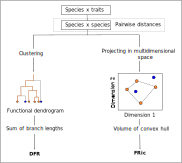
\includegraphics[scale=0.5]{figures/chapter3/DFR_FRic_chart}
\caption[Conceptual frameworks for calculating two different functional richness indices: FRic and DFR]{\textbf{Conceptual frameworks for calculating two different functional richness indices: FRic \citep{Villeger2008} and DFR \citep{Petchey2002}}. DFR (dendrogram-based functional richness) is based on the clustering of a pairwise distance matrix summarising functional dissimilarities across species. This results in the obtention of a functional dendrogram, where each tip is a species and branch lengths reflect the functional distance among all species. DFR is calculated as the sum of the branch lengths for species in a given community (for example, orange dots). FRic (volume-based functional richness) is based on the projection of species in a multidimensional space. Species relative position in the space reflects the functional distances. FRic is the volume of the convex hull that includes species in a given community.} 
\label{chartFR_calc}
\end{figure}


\subsubsection{Functional dispersion and Rao's quadratic entropy.}
Functional dispersion \citep{Laliberte2010} and Rao's quadratic entropy \citep{Rao1982, Botta-Dukat2009} are two highly correlated indices, that both aim to describe the spread of the species in the multidimensional trait space. 
Both indices are, by construction, independent from species richness \citep{Schleuter2010}. Both can take into account species relative abundance or presence-absence.

Functional dispersion is calculated as the mean distance, in the multidimensional trait space, of each species to the centroid of all species (Figure \ref{chartFDis} and Equation \ref{eqFDis}). It is expressed as:
\begin{equation}
FDis=\frac{\sum_{i} p_{i}\cdot z_{i}}{\sum_{i} p_i},
\label{eqFDis}
\end{equation}
where $p_{i}$ is the relative abundance of the $i^{th}$ species and $z_i$ the distance of the $i^{th}$ species to the centroid of all species. See \citet{Laliberte2010} for more details. 

\begin{figure}[h!]
\centering
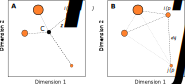
\includegraphics[scale=0.65]{figures/chapter3/FDis/chartFDis}
\caption[Conceptual framework for the calculation of functional dispersion and Rao's quadratic entropy]{\textbf{Conceptual framework for the calculation of functional dispersion and Rao's quadratic entropy.} Each orange circle represents a species, positioned in a bi-dimensional trait space. \textbf{(A) Functional dispersion}. The black point C represents the centroid of all species (its position depends on whether the calculations are abundance-weighted or not; see for more details). For the $i^{th}$ species, $z_{i}$ is the distance to the centroid. The functional dispersion is the mean distance of all species to the centroid (and can be weighted by the relative abundance of each species, $p_i$).  \textbf{(B) Rao's quadratic entropy}. $d_{i,j}$ is the pairwise distance between species \textit{i} and \textit{j}. Rao's quadratic entropy is the sum of pairwise distances weighted by the product of pairwise relative abundances.}
\label{chartFDis}
\end{figure}

Rao's quadratic entropy describes the average functional distance among species. It is conceptually similar to functional dispersion, but its calculation relies on the functional distance within each species pair rather than on distances to the centroid. Rao's quadratic entropy is expressed as:
\begin{equation}
Q=\sum_{i, j} p_{i}\cdot  p_{j} \cdot d_{i,j}, 
\label{eqFDis}
\end{equation}
where $p_{i}$ is the relative abundance of the $i^{th}$ species, $p_{j}$ the relative abundance of the $j^{th}$ species and $d_{i,j}$ is the functional distance between species $i$ and $j$, obtained from the species$\times$species distance matrix. 

\subsubsection{Functional redundancy.}
Here, I used the framework developed by \citet{Ricotta2016} to calculate the functional redundancy of an ecological community. \citet{Ricotta2016} derived an index to estimate functional redundancy from Rao's quadratic entropy and from the Simpson's diversity index. Functional redundancy is expressed as:
\begin{equation}
R=1-\frac{Q}{D},
\label{eqFRed}
\end{equation} 
where $Q$ is Rao's quadratic entropy and $D$ is Simpson's diversity index:
\begin{equation}
D=\sum_{i}p_{i}(1-p_{i}),
\end{equation} 
where $p_{i}$ is the relative abundance of the $i^{th}$ species in the community.

\subsection{Calculation of functional diversity indices}

\subsubsection{Trait selection.}
In Chapter 2, I collected and imputed the values of nine traits across terrestrial vertebrates (as well as range size). I used these data here to calculate the functional diversity indices. A crucial step was to select the traits to include in the calculations. Indeed, functional diversity indices can be sensitive to the number of traits included \citep{Mouillot2014, Cadotte2011}. A larger number of traits allows to detect functional differences among species that could be missed with fewer traits \citep{Petchey2002}. Not including enough traits may lead to missing important areas in the multidimensional trait space. On the other hand, the inclusion of correlated traits or neutral traits can inflate functional metrics or cause them to artificially converge with species diversity metrics \citep{Cadotte2011, Naeem2003}. Assessing the degree of multicollinearity among traits is thus a necessary step before calculating functional diversity indices. 

I randomly selected one imputed trait dataset among the eight imputed datasets (see Chapter 2). To improve normality, a log-10 transformation was applied to all continuous traits (except habitat breadth, which was square-rooted). Trait values were also centred and scaled to zero-mean and unit-variance across the four vertebrate classes. All traits were subsequently considered, except those relating to species diet (primary diet and diet breadth), as these were unavailable for reptiles. As such,the traits taken into consideration were: body mass; longevity; litter/clutch size; habitat breadth; habitat specialisation; diel activity; and trophic level.

\paragraph{Ecological relevance of the traits.} All the traits that were considered impacted the transfer of matter and energy across the biotic and abiotic components of a given ecosystem. As such, they were all effect traits in a broad sense. I did not aim to target a specific ecosystem function here.

\subparagraph{Body mass.} Body mass strongly impacts food-web structure and dynamics. Many underlying physiological functions and rates scale with body mass. It is as such a key determinant of energy flow within ecosystems \citep{Thompson2012,Malhi2016, Harfoot2014, Gillooly2001}.

\subparagraph{Trophic level.} Trophic level is a key determinant of ecosystem processes. Trophic level captures how species acquire resources. It is well documented that a modification in the number of trophic levels (alteration of the food chain length) strongly affects ecosystem processes through direct and indirect modifications of multitrophic interactions \citep{Duffy2007, Duffy2003, Thebault2003}. 
 
\subparagraph{Longevity and litter/clutch size.} Both longevity (which relates to the turnover of generations) and litter/clutch size characterise species reproductive output. Reproductive output is an important determinant of food web dynamics \citep{Chase1999, Hartvig2011}, and as such a key determinant of energy transfers.

\subparagraph{Diel activity.} Diel activity characterises the timing of resource acquisition. The nocturnal/non-nocturnal division notably represents the temporal resource partitioning that facilitates the coexistence of competitors \citep{Fox2011}. 

\subparagraph{Habitat breadth and natural habitat specialisation.} Habitat breadth and degree of habitat specialisation relate to species' abilities to acquire resources in different habitat types. As such, habitat breadth and specialisation characterise whether species are likely to contribute to energy transfers in a wide range of habitats, or whether their functional influence will be restricted to a small number of habitats. Habitat breadth and specialisation hence capture the potential spatial extent of resource acquisition.
 

\paragraph{Assessing the degree of multicollinearity across traits.}
To first assess whether multicollinearity could be a problem, I estimated Pearson's pairwise correlation coefficients among continuous traits, as high correlation coefficients can be an indicator of collinearity. A threshold of 0.7 is usually used for detecting potential collinearity \citep{Dormann2013}. The determinant of the correlation matrix can also be assessed, with values close to 0 indicating high degrees of multicollinearity \citep{Dormann2013}.

Table \ref{corcont} shows the pairwise correlation coefficients among continuous traits. Body mass and longevity were the two variables that had the highest correlation coefficient (0.51). The determinant of the correlation matrix was 0.67, thus indicating that the degree of multicollinearity was likely to be low among continuous traits. 
\vskip 0.5cm
\begin{table}[!htbp] \centering 
\renewcommand{\baselinestretch}{1}
\renewcommand{\arraystretch}{1.2}
\begin{center}\fontsize{9}{11}\selectfont
  \caption[Pearson's pairwise correlation coefficients among continuous traits]{\textbf{Pearson's pairwise correlation coefficients among continuous traits.} Overall, continuous traits were weakly or moderately correlated. Body mass and longevity had the highest correlation coefficient (0.51), which did not exceed the threshold value of 0.7 used across diverse field as an indicator of problematic collinearity. The determinant of the correlation matrix was 0.67, indicating that multicollinearity was likely not to be problematic among continuous traits.} 
  \label{corcont} 
\begin{tabular}{@{\extracolsep{5pt}} lcccc} 
\\[-1.8ex]\hline 
\hline \\[-1.8ex] 
 & Body mass & Longevity & Litter/clutch size & Habitat breadth \\ 
\hline \\[-1.8ex] 
Body mass & $1$ & $$ & $$ & $$ \\ 
Longevity & $0.509$ & $1$ & $$ & $$ \\ 
Litter/clutch size & $$-$0.146$ & $$-$0.083$ & $1$ & $$ \\ 
Habitat breadth & $0.167$ & $0.134$ & $0.194$ & $1$ \\ 
\hline \\[-1.8ex] 
\end{tabular} 
\end{center}
\end{table}

Nevertheless, the previous diagnostics did not take into consideration categorical traits. Potential associations between categorical and continuous traits, or among categorical traits, also needed to be assessed. To that end, I used generalised variance inflation factors (GVIF) or variance inflation factors (VIF), as developed by \citep{Fox1992}, to detect multicollinearity across all traits. Given a regression model, variance inflation factors quantify the overestimation in the variance of estimated regression coefficients due to multicollinearity among the predictors. A VIF or GVIF value of 5 or 10 is commonly used as a threshold to select out collinear predictors \citep{Dormann2013}. I used the function stepwise.vif of the R package Rnalytica \citep{Rnalytica}, in which a normally-distributed dummy variable was used as a dependent variable in a linear regression model where all traits were used as predictors. The VIF or GVIF of each predictor was then assessed.  Multicollinearity across predictors was not detected to be problematically high, as all predictors had a VIF or GVIF value below 2 (Table \ref{GVIF}). As such, all the traits figuring in Table \ref{GVIF} were included in the calculations of functional indices. 

% https://www.rdocumentation.org/packages/pedometrics/versions/0.6-6/topics/stepVIF
%% Table GVIF values among traits
\begin{table}[!h]
\renewcommand{\baselinestretch}{1}
\renewcommand{\arraystretch}{1.2}
\begin{center}\fontsize{9}{11}\selectfont
  \caption[Variance inflation factor of estimated regression coefficients for each trait treated as a predictor in a linear regression model.]{\textbf{Variance inflation factor of estimated regression coefficients for each trait treated as a predictor in a linear regression model.} For categorical traits, the GVIF was calculated rather than the VIF. All traits had a VIF or GVIF below 2: multicollinearity was not problematic among all traits.} 
  \label{GVIF} 
\begin{tabular}{@{\extracolsep{5pt}} lc} 
\\[-1ex]\hline 
\hline \\[-1.8ex] 
 Predictor & VIF or GVIF \\ 
\hline \\[-1.8ex] 
Diel activity & $1.145$ \\ 
Litter/clutch size & $1.267$ \\ 
Trophic level & $1.288$ \\ 
Specialisation & $1.391$ \\ 
Longevity & $1.441$ \\ 
Habitat breadth & $1.473$ \\ 
Body mass & $1.584$ \\ 
\hline \\[-1.8ex] 
\end{tabular} 
\end{center}
\end{table} 

\subsubsection{Calculation of functional diversity metrics across PREDICTS vertebrate communities.}

\paragraph{Overview.}
Functional diversity indices were calculated for each local vertebrate community of the PREDICTS database (in other words, for each PREDICTS site, Figure  \ref{FDcalc_chart}A). Functional richness indices (DFR and FRic) were calculated across the 180 studies for which species occurrence was available. Functional dispersion, Rao's quadratic entropy and functional redundancy were abundance-weighted, and calculated over the 132 studies which provided species relative abundance.
 
\paragraph{Implementation details.}
Previous to the calculations of the functional indices, a Gower distance matrix was computed from the species$\times$trait dataset containing all terrestrial vertebrates, using the gowdis function (FD package: \citet{Laliberte2010, Laliberte2015}). Gower distances allowed to include mixed type variables in the computation. As such, the pairwise dissimilarities among 34,377 terrestrial vertebrates was calculated. This distance matrix was then sub-setted for the species figuring in the PREDICTS database (using the dist$\textunderscore$subset function of the usedist package: \citet{usedist}).

\subparagraph{Dendrogram-based functional richness.} For the calculation of DFR, the Gower distance matrix was clustered into a functional dendrogram, using the function hclust (base R). I selected the UPGMA clustering algorithm (unweighted pair group method with arithmetic mean). This method provided the best correlation coefficient between cophenetic distances and original distances in the Gower distance matrix, of all the methods proposed in the hclust function. Then, for each PREDICTS community, the total branch length of the functional dendrogram corresponding to species in the assemblage was calculated using treedive (vegan package: \citet{vegan}). 

\textbf{NB:} Several clustering methods were provided in the hclust function. I clustered the distance matrix using all the methods and calculated cophenetic distances for each. I then calculated the correlation coefficients between cophenetic distances and Gower distances. The correlation coefficients indicated how well each of the clustering methods conserved the species$\times$species distances. The UPGMA method had the best correlation coefficient (0.82). The same method was notably employed by \citet{Flynn2009}.

\subparagraph{Volume based functional richness, functional dispersion and Rao's quadratic entropy.} FRic, FDis and Q were calculated for each site using the FD package \citep{Laliberte2015}. The Gower distance matrix was directly passed as an argument in this function. In complement, I calculated the Simpson's diversity index; I then combined Rao's quadratic entropy and the Simpson's index to estimate functional redundancy (Equation \ref{eqFRed}). 

\subsection{Assessing the impacts of land-use change on functional diversity indices}

Functional diversity metrics, notably those aiming at estimating functional richness, can be correlated with species richness. For such indices, disentangling the effects of species richness from the effects of land-use is vital, particularly because land-use change has been shown to negatively impact species richness \citep{Newbold2015}. For indices that do not correlate with species richness, the mean effects of land-use on the metrics can be directly estimated.

	\subsubsection{Functional indices independent from species richness.}
As expected by construction, functional dispersion, Rao's quadratic entropy and functional redundancy were not strongly correlated with species richness (Table \ref{cordis}). Surprisingly, volume-based functional richness was also not strongly correlated with species richness (Table \ref{corFR}, Figure \ref{SR_FR_points}A). There was hence no need to disentangle the effects of land-use from the effects of species richness on these indices. The impact of land-use was assessed using mixed-effect models (lme4 package: \citet{lme4}), specified as follows: $\textsf{Metric} \sim \textsf{Land-use} + \textsf{RE}$, where $\textsf{Land-use}$ was the recorded predominant land-use in each site, and $\textsf{RE}$ all random effects. To account for variation in experimental design across studies, the random effects included the identity of each study and block, as well as the class of vertebrates considered in each study (Table \ref{class_compo}).

	\subsubsection{Functional indices dependent on species richness.}
Dendrogram-based functional richness was highly correlated with species richness (Table \ref{corFR}, Figure \ref{SR_FR_points}B). Consequently, it was not possible to directly assess the impacts of land-use change on DFR, as decreases in species richness along the land-use gradient could have confounding effects. To overcome this problem, different studies have investigated how the species richness--functional richness relationship is affected by a disturbance of interest. I used the same approach here.

% correlation coefficients for DFR, FRic and log(SR)
\begin{table}[h!]
\renewcommand{\baselinestretch}{1}
\renewcommand{\arraystretch}{1.2}
\begin{center}\fontsize{9}{11}\selectfont
  \caption[Pearson's correlation coefficients between species richness and indices estimating functional richness]{\textbf{Pearson's correlation coefficients between species richness and indices estimating functional richness.} Volume-based functional richness (FRic) was not strongly correlated with species richness. On the other hand, the correlation between species richness and dendrogram-based functional richness (DFR) was higher. DFR and FRic were not strongly associated.} 
  \label{corFR} 
\begin{tabular}{@{\extracolsep{5pt}} cccc} 
\\[-1.8ex]\hline 
\hline \\[-1.8ex] 
 & DFR & FRic & log(SR) \\ 
\hline \\[-1.8ex] 
DFR & $1$ & $ $ & $ $ \\ 
FRic & $0.46$ & $1$ & $ $ \\ 
log(SR) & $0.71$ & $0.26$ & $1$ \\ 
\hline \\[-1.8ex] 
\end{tabular} 
\end{center}
\end{table} 


\begin{figure}[h!]
\centering
\includegraphics[scale=0.5]{figures/chapter3/SR_metrics/Richness}
\caption[Functional richness against species richness]{\textbf{Functional richness against species richness.} \textbf{(A) FRic}. FRic appeared to be independent from species richness. FRic was standardised so as to be constrained between 0 and 1. \textbf{(B) DFR}. DFR and species richness appeared to be positively associated. By definition, the functional richness for communities with only one species was 0.}
\label{SR_FR_points}
\end{figure}


% correlation coefficients for the other metrics (multivariate dispersion and redundancy)
\begin{table}[h!]
\renewcommand{\baselinestretch}{1}
\renewcommand{\arraystretch}{1.2}
\begin{center}\fontsize{9}{11}\selectfont
  \caption[Pearson's correlation coefficients between species richness and indices estimating multivariate functional spread.]{\textbf{Pearson's correlation coefficients between species richness and indices estimating multivariate functional spread.} As expected by construction, the correlation coefficients between functional dispersion, Rao's quadratic entropy, functional redundancy and species richness were small. FDis and Q were expectedly strongly correlated. Here, all functional indices were abundance-weighted.} 
  \label{cordis} 
\begin{tabular}{@{\extracolsep{5pt}} ccccc} 
\\[-1.8ex]\hline 
\hline \\[-1.8ex] 
 & FDis & Q & Redundancy & log(SR) \\ 
\hline \\[-1.8ex] 
FDis & $1$ & $ $ & $ $ & $ $ \\ 
Q & $0.94$ & $1$ & $ $ & $ $ \\ 
Redundancy & $$-$0.82$ & $$-$0.91$ & $1$ & $ $ \\ 
log(SR) & $0.27$ & $0.17$ & $0.07$ & $1$ \\ 
\hline \\[-1.8ex] 
\end{tabular} 
\end{center}
\end{table} 

\begin{figure}[h!]
\centering
\includegraphics[scale=0.8]{figures/chapter3/SR_metrics/Multivariate_spread}
\caption[Functional dispersion, Rao's quadratic entropy and functional redundancy against species richness]{\textbf{Functional dispersion, Rao's quadratic entropy and functional redundancy against species richness.} \textbf{(A) Functional dispersion}.  \textbf{(B) Rao's quadratic entropy}. \textbf{(C) Functional redundancy}. All three indices were not associated with species richness. Due to their conceptual similarity and high correlation, the behaviour of functional dispersion and Rao's quadratic entropy was similar against species richness. Functional redundancy was closely associated to both dispersion and Rao's quadratic entropy by construction.}
\label{SR_FR_points}
\end{figure}



\paragraph{How does land-use change impact the species richness--DFR relationship?}
Species richness was log-transformed to improve normality and linearity. I then investigated how land-use change affected the slope of the species richness--DFR relationship.  To that end, I used a mixed-effect model written as follows:  
$\textsf{DFR} \sim \textsf{log(SR)} + \textsf{Land-use} + \textsf{log(SR):Land-use} + \textsf{RE}$. Land-use was added as a main effect with interaction with species richness: the model allowed land-use to affect both the estimated intercept and slope of the relationship between functional and species richness. By definition, the dendrogram-based functional richness of a community with a richness of one is 0. As such, I did not focus on interpreting the estimated intercepts, as they were not ecologically meaningful. 
The estimated slopes were the focus of this analysis. According to the hypotheses presented in the introduction, I expected to observe decreases in the slope of the relationship between species richness and DFR along the land-use gradient (Figure \ref{DFRchart}). Indeed, this would signify that with a similar increase in species richness, more disturbed environments gain new functions at lower rates than more pristine environments. In other words, this would mean that species are more functionally redundant in more disturbed land-uses. Moreover, for a given species richness, the theory would then predict that the functional richness in pristine habitats is higher than in perturbed habitats (given a similar intercept).

\begin{figure}[h!]
\centering
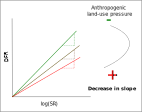
\includegraphics[scale=0.6]{figures/chapter3/DFR/DFRchart}
\caption[Expectations for the effect of land-use change on the DFR--species richness relationship]{\textbf{Expectations for the effect of land-use change on the DFR--species richness relationship.} As by construction, the DFR of a community with only one species is 0, interpreting the effect of land-use on the estimated intercept of the DFR--species richness relationship was not relevant. On the other hand, by affecting the slope of the relationship, land-use change could impact on the functional redundancy of vertebrate communities. Indeed, higher slopes signify that new functions are gained or lost at higher rates with a variation in species richness. I hypothesized that land-use change leads to increases in the functional redundancy of vertebrate communities. As such, I expected decreases in the estimated slope of the DFR--species relationship along an increasingly disturbed land-use gradient.}
\label{DFRchart}
\end{figure}

\paragraph{Disentangling the effects of species richness from the effects of land-use on functional diversity indices through simulations: an adequate approach with PREDICTS?}

\subparagraph{Approach.}
Above, I detailed how investigating how land-use change affects the species richness -- functional index relationship allows to overcome the `species richness problem' stemming from a high correlation between species richness and the metric of interest. Here, I focus on an alternative approach, classically used in diverse studies, to disentangle the effects of species richness from the effects of land-use change.

This approach is based on the randomisation of the species composition of local assemblages.  It is based upon the formulation of null expectations.  Given a species richness, randomising community composition \textit{m} times allows to generate a distribution of null expectations for a given functional index. These null expectations can then be compared to the empirical (observed) values. Along a species richness gradient that relates to a land-use gradient, such an approach allows to disentangle the impacts of land-use independently from the impacts of species richness on the calculated metrics. Here, such an approach was not necessary \textit{per se}, as most indices were independent from species richness by construction; and for DFR, I focused on the relationship between species richness and the index. Nevertheless, I implemented a simulation approach aiming at examining whether it would be a suitable method given the PREDICTS database.

Specifically, the community composition in each site was randomised by re-sampling species in the corresponding study's species pool, maintaining the species richness of each site (Figure \ref{FDcalc_chart}). Community composition was randomised 1000 times (for metrics calculated with dbFD) or 10,000 times (for DFR). For each randomised community in each site, the functional diversity indices were calculated. Null expectations of functional diversity indices were then generated for each site by taking the median value obtained across simulations.

Although only DFR was strongly correlated with species richness, I implemented this simulation approach for all functional indices that I considered. The effects of land-use were assessed using the mixed effect models detailed above. My expectations were that:
\begin{itemize}
\item For indices independent from species richness by construction, or uncorrelated with species richness, (FDis, Q and FRic), the mean values should be similar among land-uses. Specifically, the mean value expected for primary vegetation, the most pristine land-use type in the dataset, should not differ from the mean value expected in other land-uses (\textit{expectation 1}).
\item For the index that correlated with species richness (DFR), the slope of the metric--species richness relationship should be similar across land-uses (\textit{expectation 2}). 
\end{itemize} 

\textbf{NB:} For the simulations, FDis and Q were not abundance-weighted, as the simulations were based upon the randomisation of species presence-absence. 

\begin{figure}[h!]
\centering
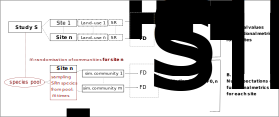
\includegraphics[scale=0.60]{figures/chapter3/chart_FD_calculations}
\caption[Design for calculating functional indices and null expectations for PREDICTS sites]{\textbf{Design for calculating functional indices and null expectations for PREDICTS sites.} \textbf{(A)} Empirical values for the functional diversity indices were obtained for each PREDICTS site, nested within studies. Each site was characterised by its species richness and its land-use. \textbf{(B)} For a given site \textit{n} of richness SR$_{n}$, the community composition was randomised \textit{m} times by drawing SR$_{n}$ species from the study's species pool. Null expectations for the site \textit{n} were then obtained by taking the median value of the indices across simulations.}
\label{FDcalc_chart}
\end{figure}

\subparagraph{Simulation results, and hypotheses as to why simulations may be inadequate.}
Simulation results showed that land-use was having an effect on null expectations, even for indices independent from species richness by construction (Figure \ref{simresults}). A significant decrease in the mean effect was observed for FRic, FDis and Q in a number of land-uses, contradicting \textit{expectation 1}. Moreover, a significant decrease in the slope of the DFR--species richness relationship was observed for all land-uses except mature secondary vegetation, contradicting \textit{expectation 2}. 

Hereafter, I propose a mechanism that may explain why simulated results differed from \textit{expectations }1 and \textit{2}. Simulations were based on the randomisation of the species composition of each site. Species were drawn at random from the species pool, defined as the set of species in each study (equivalent to a `regional' species pool). As such, simulations were sensitive to the composition of the species pool. Nevertheless, the PREDICTS database has an imbalanced design, such that each study do not have sites in all of the land-uses. This may be constricting species pools in some cases. For instance, for a site of land-use `Pasture' belonging to a study where primary vegetation was also sampled, the species pool may be bigger than for a site of land-use `Pasture' where only pasture and plantation forest were sampled. As such, biases in species pool may influence simulation results. Simulation results may capture trends reflecting differences in the size and composition of species pool (Figure \ref{speciespool}), which may explain the patterns observed in Figure \ref{simresults}. 

\begin{figure}[h!]
\centering
\includegraphics[scale=0.70]{figures/chapter3/Simulations/p_sim}
\caption[Simulation results.]{\textbf{Simulation results.} Here, null expectations for each index were generated by randomising species presence-absence in each site, maintaining the local species richness. Species were drawn at random from a `regional' pool of species corresponding to all species sampled within studies. In theory, land-use should not have any effect on simulated values. Contrary to this expectation, land-use had a significant effect on the simulated values of all functional metrics for a number of land-uses. As such, I questioned the validity of the simulation approach employed here.}
\label{simresults}
\end{figure}

\subparagraph{Simulation approach: conclusion.} The imbalanced design of the PREDICTS database may be causing biases in species pool, which may render simulation approaches difficult to interpret. As such, the simulation approach was not developed further here. For that reason, simulation results are not detailed in the Results section below.

\begin{figure}[h!]
\centering
\includegraphics[scale=0.70]{figures/chapter3/Simulations/pool_species_FDis}
\caption[]{\textbf{(A) Size distribution of species pools in each land-use and (B) distribution of the functional dispersion of the species pools.)} The trend observed in the simulation results may reflect differences in the composition of study's species pools. For instance, the median functional dispersion of the species pools corresponding to urban land-uses was smaller than the median functional dispersion of the species pools in other land-uses.}
\label{speciespool}
\end{figure}


\pagebreak
\section{Results}

\subsection{Land-use change constricted the functional richness of assemblages}
Land-use had a significant effect on volume-based functional richness (Figure \ref{LU_mean_FRic}). For mature and intermediate secondary vegetation, the mean functional richness was similar to that of primary vegetation. For all other more disturbed land-uses, mean functional richness was significantly different from the mean functional richness of primary vegetation, and decreased with increasing land-use disturbance. 
% Even though not significantly different, the mean functional richness for mature secondary vegetation was higher than the mean functional richness for primary vegetation. 

\begin{figure}[h!]
\centering
\includegraphics[scale=0.70]{figures/chapter3/FRic/Mean_effect_LU}
\caption[Mean effect of land-use on the volume-based functional richness of vertebrate communities (FRic)]{\textbf{Mean effect of land-use on the volume-based functional richness of vertebrate communities (FRic).} \textbf{PV:} primary vegetation; \textbf{MSV:} mature secondary vegetation; \textbf{ISV:} intermediate secondary vegetation; \textbf{YSV:} young secondary vegetation; \textbf{PF:} plantation forest; \textbf{CR:} cropland; \textbf{UR:} urban.}
\label{LU_mean_FRic}
\end{figure}


\subsection{Land-use change promoted the functional homogenisation of local vertebrate communities}

\subsubsection{Land-use change reduced multivariate functional dispersion.}

Land-use significantly impacted the functional dispersion of vertebrate communities: for all agricultural and urban land-uses, mean functional dispersion was significantly lower than for primary and secondary vegetation (Figure \ref{LU_mean_FDis}). For mature and intermediate secondary vegetation, mean functional dispersion, even though not significantly different, was higher than the mean functional dispersion for primary vegetation. \\ 
\textbf{NB:} The mean effect of land-use on Rao's quadratic entropy was similar to the mean effect of land-use on functional dispersion. This was expected due to the high correlation between these two indices. The plot for Rao's quadratic entropy figures in the SI.

\begin{figure}[h!]
\centering
\includegraphics[scale=0.70]{figures/chapter3/FDis/Mean_effect}
\caption[Mean effects of land-use on the functional dispersion of local vertebrate communities]{\textbf{Mean effects of land-use on the functional dispersion of local vertebrate communities (FDis).} \textbf{PV:} primary vegetation; \textbf{MSV:} mature secondary vegetation; \textbf{ISV:} intermediate secondary vegetation; \textbf{YSV:} young secondary vegetation; \textbf{PF:} plantation forest; \textbf{CR:} cropland; \textbf{UR:} urban.}
\label{LU_mean_FDis}
\end{figure}


\subsubsection{Land-use change enhances the functional redundancy of local vertebrate communities.}

\paragraph{Functional redundancy derived from Rao's quadratic entropy and the Simpson's diversity index.}
Here, functional redundancy was calculated from Rao's quadratic entropy and the Simpson's diversity index \citep{Ricotta2016}. The mean functional redundancy was only significantly higher than that of primary vegetation in urban land-uses ((Figure \ref{LU_mean_FRedundancy})). For mature and intermediate secondary vegetation, the mean functional redundancy was lower than the mean functional redundancy of primary vegetation, even though the difference was not significant.

\begin{figure}[h!]
\centering
\includegraphics[scale=0.70]{figures/chapter3/FRedundancy/Mean_effect_LU}
\caption[Mean effect of land-use on the functional redundancy of vertebrate communities]{\textbf{Mean effect of land-use on the functional redundancy of vertebrate communities.} \textbf{PV:} primary vegetation; \textbf{MSV:} mature secondary vegetation; \textbf{ISV:} intermediate secondary vegetation; \textbf{YSV:} young secondary vegetation; \textbf{PF:} plantation forest; \textbf{CR:} cropland; \textbf{UR:} urban.}
\label{LU_mean_FRedundancy}
\end{figure}

\paragraph{Functional redundancy inferred from the slope of the functional-richness -- species richness relationship.} Here, I investigated how land-use affected the slope of the DFR--species richness relationship. For all secondary vegetation, as well as for agricultural and urban land-uses, the slope of the relationship was significantly lower than the slope estimated for primary vegetation (Figures \ref{slopesDFR} and \ref{reglines}). There was a trend for slopes to decline with increasing land-use disturbance (Figure \ref{slopesDFR}). 

Global land-use change hence impacted the rate at which the functional distance among species (measured from  functional dendrograms) accumulated in local communities with increases in local species richness.

The two approaches used to estimate functional redundancy gave different insights. Notably, the functional redundancy estimated with the metrics developed by \citep{Ricotta2016} was only detected to significantly increase in urban land-uses. On the other hand, functional redundancy as inferred from the species richness-- was estimated to be significantly highest in pastures, using the second approach, and significantly different from that of primary vegetation in all land-uses except mature secondary vegetation.

Figure \ref{reglines} also showed that, given a species richness, the functional richness of disturbed land-uses was predicted to be significantly lower than that of primary vegetation (given the differing slopes). 

\vspace{1cm}
\begin{figure}[h!]
\centering
\includegraphics[scale=0.70]{figures/chapter3/DFR/Mean_effect}
\caption[Effect of land-use on the slope of the relationship between species richness and dendrogram-based functional richness]{\textbf{Effect of land-use on the slope of the relationship between species richness and dendrogram-based functional richness.} \textbf{PV:} primary vegetation; \textbf{MSV:} mature secondary vegetation; \textbf{ISV:} intermediate secondary vegetation; \textbf{YSV:} young secondary vegetation; \textbf{PF:} plantation forest; \textbf{CR:} cropland; \textbf{UR:} urban. Land-use significantly affected the slope of the species richness--functional richness relationship.}
\label{slopesDFR}
\end{figure}

% regression lines
\begin{figure}[h!]
\centering
\includegraphics[scale=0.70]{figures/chapter3/DFR/regression_lines}
\caption[Regression lines for the estimated DFR--species richness relationships]{\textbf{Regression lines for the estimated DFR--species richness relationships.} \textbf{PV:} primary vegetation; \textbf{MSV:} mature secondary vegetation; \textbf{ISV:} intermediate secondary vegetation; \textbf{YSV:} young secondary vegetation; \textbf{PF:} plantation forest; \textbf{CR:} cropland; \textbf{UR:} urban. The regression line was significantly steeper for primary vegetation. Estimated intercepts were not meaningful, as by definition the DFR of communities with only one species is 0. Variations in the slope of the relationship indicated that the rate at which the functional distance among species increased with an increase in species richness was significantly affected by land-use.}
\label{reglines}
\end{figure}

\pagebreak
\section{Discussion}
% failed simulation approaches. These results would be strnonger and validated if ... 

In this Chapter, I used a meta-analytic approach to assess how global land-use change impacted the functional diversity of local vertebrate communities. This work constituted, to my knowledge, the first attempt to tackle this question at global scales and across the four vertebrate classes simultaneously. 

I showed that globally, land-use change had significant impacts on the functional diversity of vertebrate assemblages. Land-use change acted as an environmental filter that constricted the functional breadth of local assemblages and their mean functional dispersion. 

Indeed, because volume-based functional richness is a multivariate analogue of the functional range, global land-use change significantly impacted the functional composition of local vertebrate communities by constricting the multivariate trait range (Figure \ref{LU_mean_FRic}). Species located at the periphery of the functional convex hull were more likely to be removed in disturbed land-uses. As such, land-use change significantly impacted the functional composition of local vertebrate communities by reducing the breadth of functions. Land-use change acted as an environmental filter which excluded species having combination of trait values placing them at the extremity of the communities' convex hulls. 

Global land-use change also impacted the trait composition of local vertebrate communities by reducing the mean functional distance of species to the functional centroid of all species (functional dispersion). Species were significantly closer to each other in the multidimensional trait space for agricultural and urban land-uses. These results were in agreement with results obtained for FRic: land-use change selectively removed species that were further away in the trait space, also more likely to be located at the periphery of the convex hulls. Global land-use change, by reducing multivariate functional dispersion, negatively impacted the breadth of functions in local vertebrate communities. These results show that global land-use change promoted the functional clustering of vertebrate assemblages.

Such results could be validated further with an appropriate simulation approach, allowing to generate null expectations of local functional diversity indices. Here, I showed that the simulation approach I attempted may have failed due to potential biases in regional species pool. This work could be developed further to try and design a pertinent and applicable simulation approach.

%For mature secondary vegetation, mean volume-based functional richness, mean functional dispersion and mean functional redundancy were found to be higher than those of primary vegetation, even though the differences were not significant. Such effects could be explained by the fact that these habitats could be suitable for both species found in more pristine environments, as well as for more generalist species adapted to both pristine and disturbed habitats. 

Overall, global land-use change promoted the functional homogenisation of local communities: species tended to be more functionally similar in perturbed land-uses, and the effect size tended to increase with increasing land-use disturbance. These results agree with studies conducted at local scales that showed, for example, that urbanisation impacted the range of trait values by cutting the tails of trait distributions \citep{LaSorte2018}. Nevertheless, these results contrast with one study that found no effect of urbanisation on the functional diversity of avian assemblages \citep{Hagen2017}. There is, however, more and more empirical evidence showing that land-use change favours widespread, generalist species \citep{Newbold2018a}, negatively impacts local functional diversity \citep{Chapman2018, Tinoco2018, Flynn2009, Huijbers2015}, and as such, enhances the biotic homogenisation of local communities \citep{Newbold2019_ets}.

Here, I did not investigate the mechanisms behind changes in functional composition. Land-use change could filter out species with functional attributes rendering them unable to cope with the conditions of disturbed habitats; this would correspond to a mechanism known as functional nestedness \citep{Balsega2015}. On the other hand, novel species, not found in more pristine environments, could also settle in disturbed habitats: the establishment of novel species with functional attributes rendering them able to settle in more disturbed habitats is termed functional turnover. Novel methods have been developed to assess functional nestedness and turnover \citep{Balsega2015}. They are notably based on the estimation of functional beta-diversity, which is then partitioned into a turnover and nestedness components. The present work could be developed in the future to investigate the mechanisms driving changes in the functional composition of local vertebrate communities.

By negatively impacting local functional diversity and promoting functional homogenisation, global land-use change could have deleterious effects on local ecosystem functioning \citep{Olden2004}. Functional redundancy is often presented as a safeguard for ecosystem processes. \citet{Cooke2019} found that, across mammals and birds, species-high regions had high functional redundancy and low functional dispersion. The results obtained in this work also underlined the existence of a trade-off between functional redundancy and functional dispersion. Undisturbed land-uses tended to have low redundancy coupled with high dispersion and high functional richness, whereas the opposite was observed for disturbed land-uses. As such, ecosystem processes driven by functionally vulnerable and rare species in pristine land-uses could be at risk if the landscape is modified for human purposes, given the overall lower functional redundancy of undisturbed land-uses.

Finally, in this Chapter, I did not explicitly link the functional diversity metrics to specific functional roles. Nevertheless, the traits that were included in the calculations of the indices were involved in the definition of certain ecosystem functions (for example, trophic level linked to food-web structure and energy transfers). Potential developments of this work could include building explicit links between functional diversity and specific ecosystem functions. The objective of the next Chapter is to develop future questions that I could investigate in the future years of my PhD.



